\documentclass{article}

\usepackage{blindtext}
\usepackage[francais]{babel}
\usepackage[latin1]{inputenc}
\usepackage[T1]{fontenc}
\usepackage{lmodern}
\usepackage{amsmath}
\usepackage{amssymb}
\usepackage{mathrsfs}
\usepackage{graphicx}
\usepackage{enumitem}


\title{Traitement du signal}
\author{BORDE Martin}
%\subtitle{}
\begin{document}
\maketitle

\section{Introduction}
%\blindtext

\begin{itemize}
\item 28 h de cours + 2 s\'eances de FOAD $ \rightarrow $ exercices ou d\'eveloppement 
\item ElectroCardioGramme $ \rightarrow $  Systeme Nerveux Autonome
\end{itemize}

\section{Signaux de bases}
\subsection{Sinusoide}
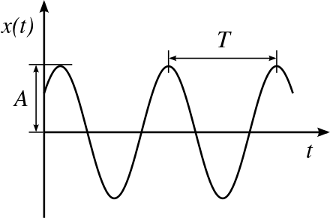
\includegraphics{img/sinus.png}
\newline \newline
D\'efinition et propri\'et\'e :
\begin{itemize}[label=\textbullet]
\item T = P\'eriode
\item A = constante
\item Acc = 2A
\item w = pulsation
\item f = 1/t (Hertz)
\item w = (2* $ \pi $ )/T
\item t0 = D\'ecalage a l'origine
\item $ \varphi $0 = phase a l'origine
\item $ \varphi $0 = w*t0
\item s(t)=Asin(wt+$\varphi$0)
\item s(t)=Asin(w(t+t0))
\end{itemize}

\subsection{Signal porte}
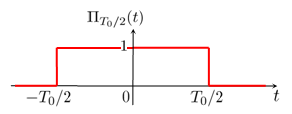
\includegraphics{img/porte.png}
\newline \newline
La fonction porte, est la fonction indicatrice de l'intervalle r\'eel [-1/2, 1/2], c'est-\`a-dire la fonction math\'ematique par laquelle un nombre r\'eel a une image nulle, sauf s'il est compris entre -1/2 et 1/2, auquel cas son image vaut 1.L'aire total sous la ligne vaut 1.

\subsection{Impulsion de Dirac}
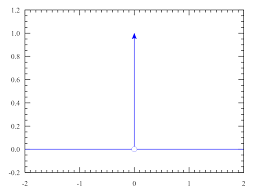
\includegraphics{img/dirac.png}
\newline \newline
La distribution de Dirac, introduite par Paul Dirac, peut \^etre informellement consid\'er\'ee comme une fonction qui prend une valeur infinie en 0, et la valeur z\'ero partout ailleurs, et dont l'int\'egrale sur R est \'egale \`a 1.
Le dirac a donc une surface de 1 , une amplitude infini et une dur\'ee de 0.
Si l'on pose plusieurs Dirac \`a la suite , on appele ce ph\'enom\`ene un peigne de Dirac.

\subsection{Peigne de Dirac}
\begin{center}
	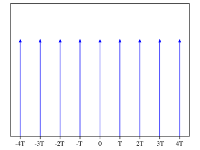
\includegraphics{img/peigne.png}
\end{center}
En math\'ematiques, la distribution peigne de Dirac, ou distribution cha , est une somme de distributions de Dirac espac\'ees de T. 
\newline \newline
\subsection{Echelon}
\begin{center}
	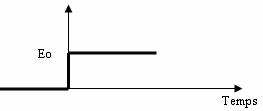
\includegraphics{img/echelon.jpg}
\end{center}
\subsection{Rampe}
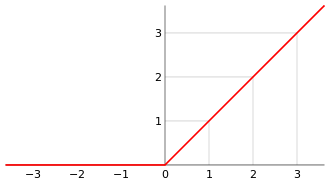
\includegraphics{img/ramp.png}
\newline \newline
\subsection{Transform\'ees miroir}
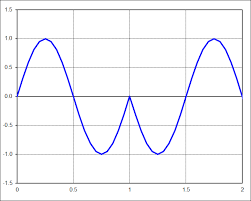
\includegraphics{img/mirror.png}
\newline \newline
S(t) $ \rightarrow $ S(-t)

\begin{center}
	\begin{tabular}{ c || c | c | c | c }
		t & -T & 0 & T & 2T \\ \hline \hline
		s(t) & 0 & 1 & 1 & 0\\ \hline
		s(t+1) & s(0)=1 & s(1)=1 & s(2)=0 & s(3)=0\\ \hline
		s(t-1) & s(-2)=0 & s(-1)=0 & s(0)=1 & s(1)=1\\\hline
	\end{tabular}
\end{center}

\section{Les s\'eries de Fourier}

\subsection{But :}
D\'ecomposer un signal en vibration.
\newline
\begin{center}
	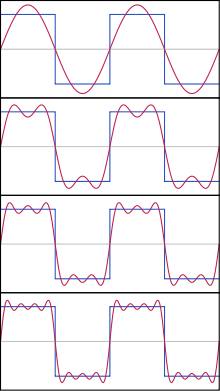
\includegraphics{img/Fourier_Series.png}
\end{center}
Premiere = fondamentale.\newline
Suivante = multiples de la fondamentale = harmonique.\newline

Possibilit\'e de recr\'eer avec triangles mais bon on le fait pas parce que pas facile.\newline
Fourier = sinusoides = plus simple.

\begin{center}$ \downarrow $\end{center}
\subsection{Repr\'esentation spectrale}
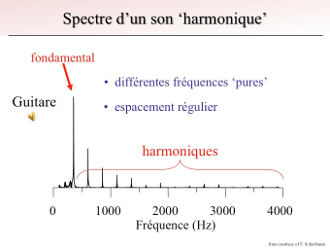
\includegraphics{img/spectre.jpg}
\newline \newline
Les diff\'erentes harmoniques repr\'esentent les diff\'erentes signaux sinusoidales ajout\'es au fur et a mesure pour approcher le signal 
Fondamentale = premier.
Harmonique = N * Fondamentale ( ou N est Entier ).
La repr\'esentation spectrale n'est pas complete car il manque le d\'ecalage.
La repr\'esentation spectrale est bien plus lisible, moins brouillon.


\section{Transform\'ees de Fourier}

\section{Num\'erique}

\section{Application}

\end{document}
